\documentclass[aspectratio=169]{beamer}
\usepackage[utf8]{inputenc}
%\usepackage[authordate,backend=biber,natbib]{biblatex-chicago}
%\usepackage{booktabs}
%\addbibresource{growthreferences.bib}

%\usepackage{utopia} %font utopia imported

\usetheme{Madrid}
\usecolortheme{beaver}

%------------------------------------------------------------
%This block of code defines the information to appear in the
%Title page
\title[Autor, Dorn, and Hanson (2016)] %optional
{The China Shock: Learning from Labor Market Adjustment to Large Changes in Trade}

\subtitle{David Autor, David Dorn, and Gordon Hanson, \emph{Annual Review of Economics}, 2016}

\author [Hauk] % (optional)
{William~R.~Hauk,~Jr.} %\inst{1} %\and J.~Doe\inst{2}} 

\institute[UofSC] % (optional)
{
  %\inst{1}%
  Darla Moore School of Business\\
  University of South Carolina
  %\and
  %\inst{2}%
  %Faculty of Chemistry\\
  %Very Famous University
}

\date[ECON 860, Fall 2021] % (optional)
{ECON 860 -- International Trade Theory\\Fall 2021}

\logo{
\includegraphics[height=1cm]{UofSC_Monogram_Stack_CMYK_G.jpg}}

%End of title page configuration block

%---------------------------------------------------------

\AtBeginSection[]
{
  \begin{frame}
    \frametitle{Table of Contents}
    \tableofcontents[currentsection,hideallsubsections]
  \end{frame}
}

%------------------------------------------------------------

\begin{document}

%The next statement creates the title page.
\frame{\titlepage}

%-------------------------------------------------------------

\section{Introduction}

%-------------------------------------------------------------

\begin{frame}{Introduction}

\begin{itemize}
    \item<1-> The standard undergraduate textbook tells us that trade is good for a country’s overall welfare.  There are distributional effects, but the gains to the winners are sufficient to compensate the losers.
    \item<2-> Strong consensus in economics towards free trade.  Even as evidence emerged in 1980s and 1990s of gaps between skilled and unskilled workers, this was explained empirically as more of a technology shock than a trade shock.
    \item<3-> Even when workers did lose their jobs due to trade, they should be able to reallocate easily to other industries.  Short-to-medium run gains from trade should be positive.
\end{itemize}
    
\end{frame}

%-------------------------------------------------------------

\begin{frame}{Figure 1}

\begin{figure}
    \centering
    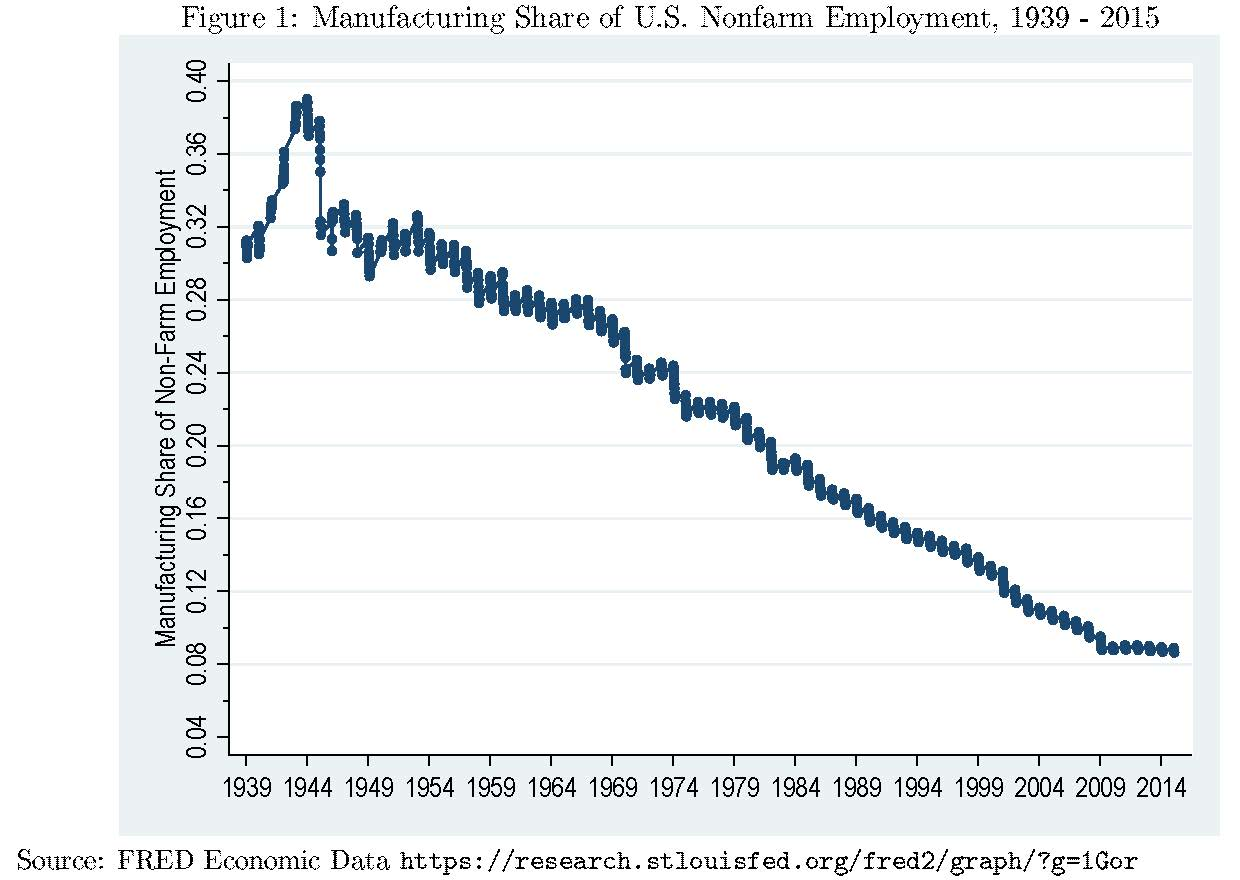
\includegraphics[scale=0.6]{AutorDornHansonFig1.jpg}
    \label{fig:fig1}
\end{figure}
    
\end{frame}

%-------------------------------------------------------------

\section{China's Rise}

%-------------------------------------------------------------

\begin{frame}{Rise of Chinese Manufacturing}

\begin{itemize}
    \item<1-> Rise of China has challenged the consensus on trade and wages.  Distributional effects (theory has recognized) and adjustment costs (theory has tended to downplay) have been relatively large.
    \item<2->  Many pundits were pessimistic about China’s chances as recently as late 1980s due to turmoil from Tiananmen Square incident
    \item<3-> Reformers gained upper hand in early 1990s, and manufacturing activity in China exploded, especially in Special Economic Zones on the east coast.  Number of SEZs increased from 20 in 1991 to 150 in 2010.
    \item<4-> Chinese share of world manufacturing exports grew from 2.3\% in 1991 to 18.8\% in 2013.  
\end{itemize}
    
\end{frame}

%-------------------------------------------------------------

\begin{frame}{Figure 2}

\begin{figure}
    \centering
    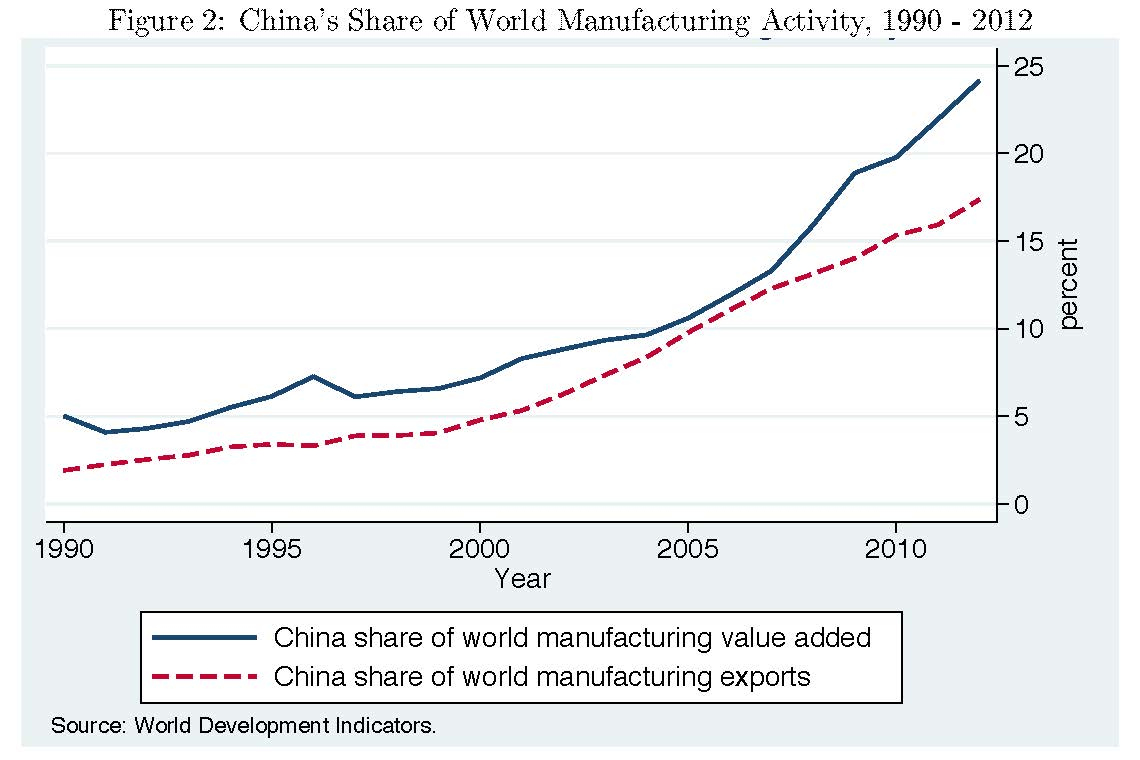
\includegraphics[scale=0.7]{AutorDornHansonFig2.jpg}
    \label{fig:fig2}
\end{figure}
    
\end{frame}

%-------------------------------------------------------------

\subsection{Making Use of Trade Shocks}

%-------------------------------------------------------------

\begin{frame}{The China ``Shock"}

\begin{itemize}
    \item<1-> Autor, Dorn, and Hanson make the argument that the Chinese transition to a manufacturing exporter owes more to internal political and economic issues in China than the global economy.  Thus, its growth is plausibly exogenous.
    \item<2-> The rise of China is importance both because of its magnitude and the relative paucity of natural experiments in international trade.  (E.g. NAFTA was caused by foreign investment as much as it caused foreign investment.)
\end{itemize}
    
\end{frame}

%-------------------------------------------------------------

\begin{frame}{Why We Should Study China}

Three features of China’s experience make it worthy of detailed study:

\begin{itemize}
    \item<1-> Unexpected nature of China’s export growth caught many people by surprise.
    \item<2-> China’s relative degree of isolation under Mao, which created a lot of opportunity for China to catch up.
    \item<3->  Manufacturing was at the heart of its economic turn-around, as opposed to raw materials – large positive supply shock in manufacturing and large demand shock for raw materials.
\end{itemize}
    
\end{frame}

%-------------------------------------------------------------

\subsection{The Global Factory}

%-------------------------------------------------------------

\begin{frame}{Figure 3.A}

\begin{figure}
    \centering
    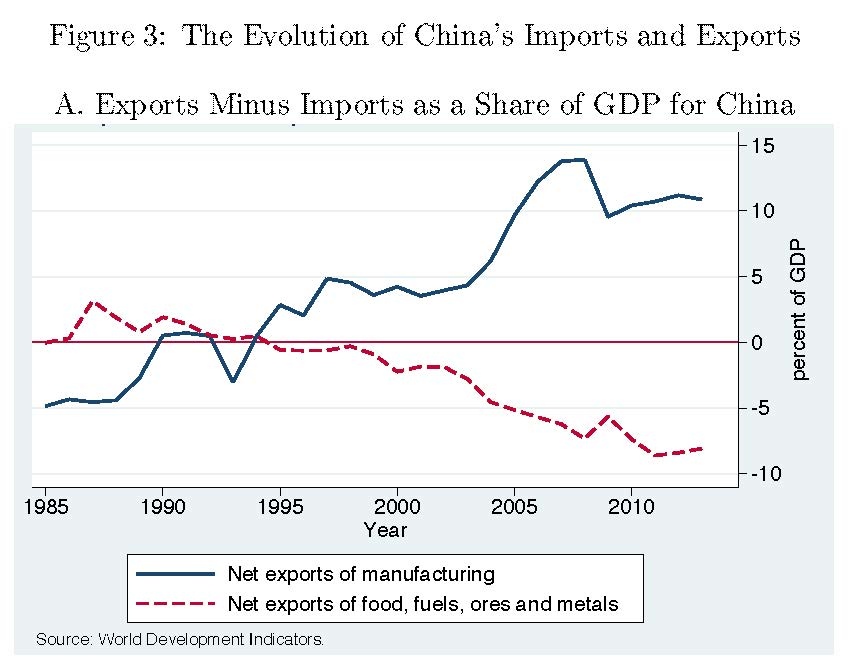
\includegraphics[scale=0.8]{AutorDornHansonFig3a.jpg}
    \label{fig:fig3a}
\end{figure}
    
\end{frame}

%-------------------------------------------------------------

\begin{frame}{Figure 3.B}

\begin{figure}
    \centering
    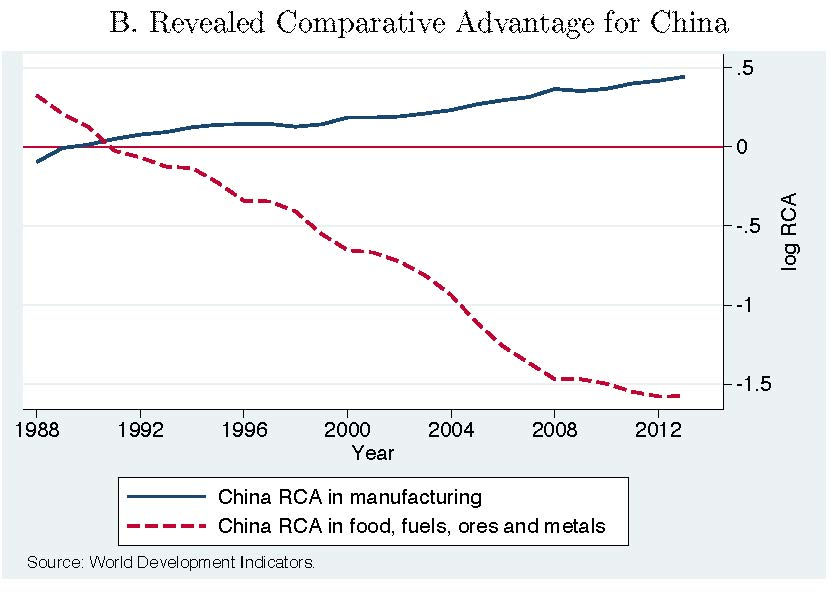
\includegraphics[scale=0.85]{AutorDornHansonFig3b.jpg}
    \label{fig:fig3b}
\end{figure}
    
\end{frame}

%-------------------------------------------------------------

\begin{frame}{The Global Factory}

\begin{itemize}
    \item<1-> China probably had a long-standing comparative advantage in manufacturing, but it remained latent during the Maoist era.  Strength only emerged in late 1980s.
    \item<2-> In 1992, China moved from a comparative disadvantage to comparative advantage in manufactures, and from a comparative advantage to disadvantage in primary products.
    \item<3-> However, as noted by Figure 4, China’s net import penetration varied substantially across industries.  Because of this variation, U.S. industries, and the regions in which they locate, vary widely in their exposure to import competition from China.
\end{itemize}
    
\end{frame}

%-------------------------------------------------------------

\begin{frame}{Figure 4}

\begin{figure}
    \centering
    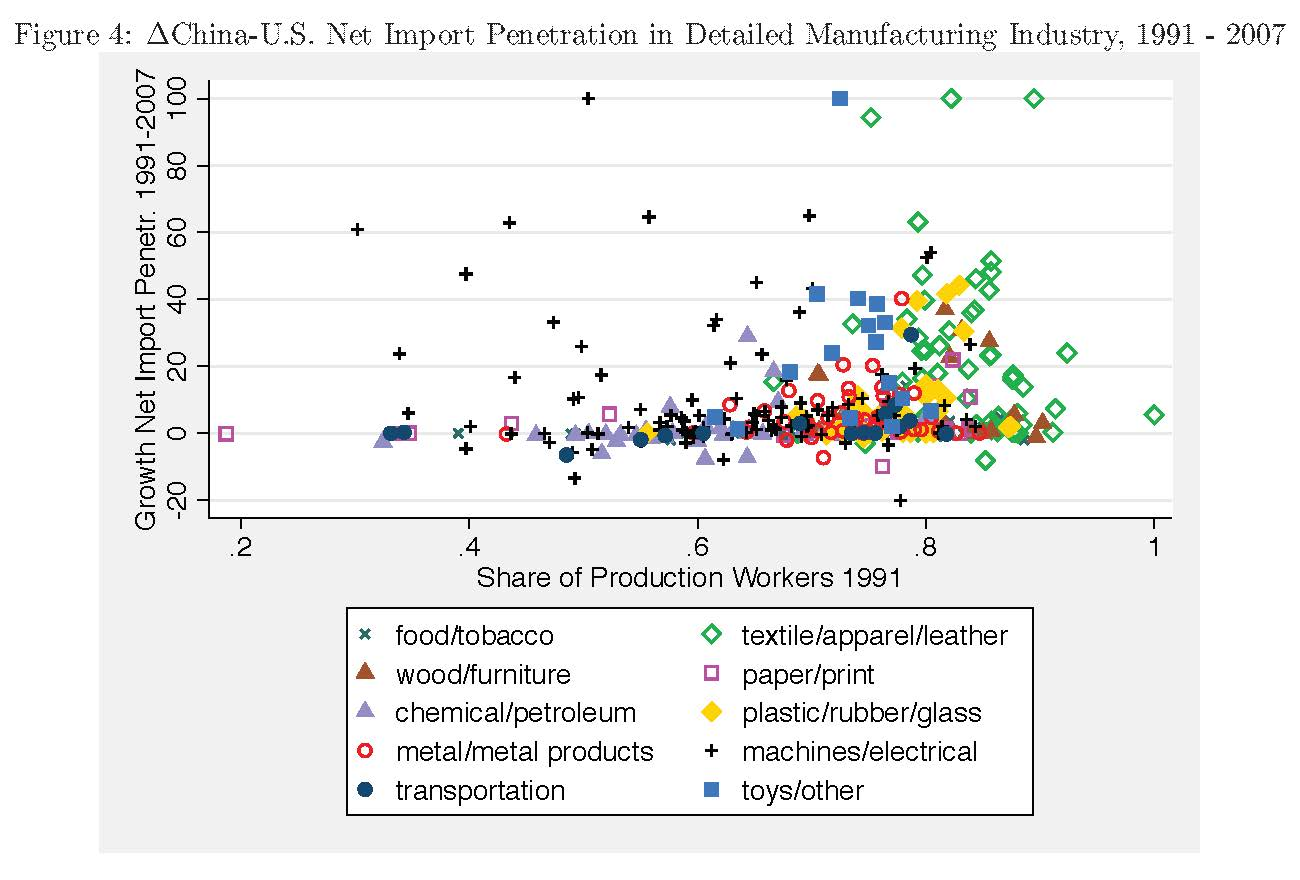
\includegraphics[scale=0.6]{AutorDornHansonFig4.jpg}
    \label{fig:fig4}
\end{figure}
    
\end{frame}

%-------------------------------------------------------------

\begin{frame}{WTO Accession 2001}

\begin{itemize}
    \item<1-> Chinese manufacturing accelerated after WTO accession in 2001.  At the same time, China had a huge surge in manufacturing productivity – pace of growth was about 8\% a year between 1998 and 2007.
    \item<2-> WTO membership meant that China liberalized many state-owned manufacturing firms and got steadier access to raw materials, helping productivity growth.
\end{itemize}
    
\end{frame}

%-------------------------------------------------------------

\subsection{The Global Macroeconomic Context}

%-------------------------------------------------------------

\begin{frame}{The Global Macroeconomic Context}

\begin{itemize}
    \item<1-> During this time period, China’s trade surplus increased substantially, while the U.S.'s worsened.
    \item<2-> Because these are the two largest economies in the world and the U.S. dollar functions as a global reserve currency, China’s trade surplus resulted in large purchases of dollar-denominated assets.
    \item<3-> Trade imbalances complicate the standard trade model.  Under balanced trade, U.S. workers shift from import-competing to export-oriented industries.
    \item<4-> With a large trade deficit, workers in import competing industries have to leave the traded goods sector and possibly the workforce entirely.
    \item<5-> At some point in the future, Chinese savings would fall, consumption would rise, and the trade flows would go in the other direction.
\end{itemize}
    
\end{frame}

%-------------------------------------------------------------

\begin{frame}{Figure 5}

\begin{figure}
    \centering
    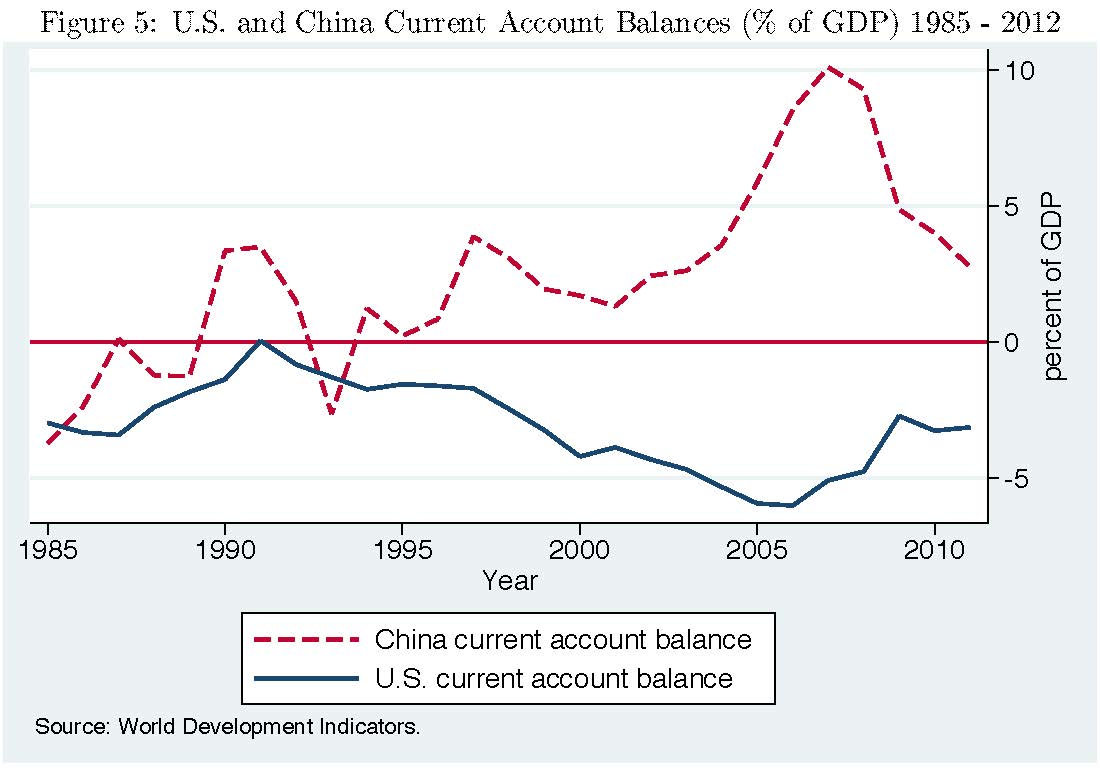
\includegraphics[scale=0.65]{AutorDornHansonFig5.jpg}
    \label{fig:fig5}
\end{figure}
    
\end{frame}

%-------------------------------------------------------------

\section{Theory}

%-------------------------------------------------------------

\begin{frame}{Theory}

\begin{itemize}
    \item<1-> Standard H-O model predicts a link between trade shocks and changes in factor returns, but this model has some shortcomings, which we have discussed previously.
    \item<2-> More recent work focuses on heterogeneous firms (e.g. Melitz (2003)).  Focus has been on the various margins through which firms adjust to trade shocks.
    \item<3-> Model proposed in this paper follows a trend of incorporating gravity-type structures, which allows for tractable descriptions of labor mobility between regions or industries.
    \item<4-> If there are frictions to worker mobility, then there are potentially several margins through which trade shocks could affect labor markets.
\end{itemize}
    
\end{frame}

%-------------------------------------------------------------

\subsection{A Bare Bones Model}

%-------------------------------------------------------------

\begin{frame}{A Bare Bones Model}

\begin{itemize}
    \item<1-> Model contains a single labor-market friction – imperfect labor mobility within the country.  Contrary to many other models, but perhaps better in tune with data.
    \item<2-> Begin with an assumption of complete geographic labor immobility.  Variation in regional exposure to foreign competition comes from differences in regional industry specializations.
\end{itemize}
    
\end{frame}

%-------------------------------------------------------------

\begin{frame}{Gravity-Like Trade}

Trade has a gravity-type structure – total demand by the U.S. aggregate economy for traded output produced in U.S. region $ i $ is:

\begin{equation}
    X_{i} = \sum_{k}\frac{A_{i,k} \tau_{i,k}^{-\theta}}{\Phi_k} E_{k}
    \label{eq:Xi}
\end{equation}

where $ A_{i,k} $ is the production capacity of industry $ k $ in region $ i $, $ \tau_{i,k} $ is an iceberg transportation cost to ship goods from region $ i $ in industry $ k $ to the U.S. market, $ \theta $ is the trade-cost elasticity, $ E_{k} $ is aggregate U.S. expenditure on industry $ k $, and $ \Phi_k = \sum_{i'} A_{i'} \tau_{i',k}^{-\theta} $ is a competitiveness index for the U.S. market in industry $ k $.
    
\end{frame}

%-------------------------------------------------------------

\begin{frame}{Change in Regional Output}

If there is a change in traded output in regions that supply the U.S., we can derive the impact on region i by totally differentiating equation (\ref{eq:Xi}):

\begin{equation}
    \hat{X}_{i} = \sum_{k} \phi_{i,k} \hat{E}_{k} - \theta \hat{w}_{i} + \sum_{k} \phi_{i,k} \hat{A}_{k} + \sum_{k} \phi_{i,k} \sum_{i' \neq c} \rho_{i',k} \hat{A}_{i',k} - \sum_{k} \phi_{i,k} \rho_{c,k} \hat{A}_{c,k}
    \label{eq:xihat}
\end{equation}

where $ c $ indexes China, $ \phi_{i,k} = \frac{X_{i,k}}{X_{i}} $ is the share of industry $ k $ in region $ i $’s total sales to the U.S. market, and $ \rho_{i,k} = X_{i,k} E_{k} $ is the share of region $ i $ in total U.S. expenditure on industry $ k $.  Also, assume that $ \hat{A}_{i,k} = \hat{A}_{k} - \theta \hat{w}_{i} $ (i.e. local productivity changes are reflected in national productivity changes and local wage changes). 
    
\end{frame}

%-------------------------------------------------------------

\begin{frame}{The China Shock}

\begin{itemize}
    \item<1-> We are primarily interested in the last part of equation (\ref{eq:xihat}), which captures the growth of China’s productive capacity on traded output in U.S. region $ i $.  Rewrite this as:
    \begin{equation}
        \sum_{k} \phi_{i,k} \rho_{c,k} \hat{A}_{c,k} = \sum_{k} \phi_{i,k} \left[ \frac{X_{c,k} \hat{A}_{c,k}}{E_{k}} \right]
        \label{eq:Chinashock}
    \end{equation}
    which is the weighted average exposure of region $ i $ to changes in U.S. industry import penetration mandated by changes in Chinese production capabilities.
    \item<2-> Because weights $ \phi_{i,k} $ vary across regions of the U.S., the exposure to Chinese traded goods varies across U.S. regions.
\end{itemize}
    
\end{frame}

%-------------------------------------------------------------

\subsection{Identifying the Reduced-Form Impact of the China Trade Shock}

%-------------------------------------------------------------

\begin{frame}{Identifying the Reduced-Form Impact of the China Trade Shock}

\begin{itemize}
    \item<1-> Estimating the impact of the trade shock in equation (\ref{eq:Chinashock}) requires that we control for confounding factors.  Fortunately, these factors are identified in equation (\ref{eq:xihat}).
    \item<2-> The first term in equation (\ref{eq:Xi}) is $ \sum_{k} \phi_{i,k} \hat{E}_{k} $, which is the regional exposure to U.S. industry demand shocks.  Reduced form regressions of regional outcomes on regional trade exposure might be contaminated by U.S. product demand shocks.
    \item<3-> Following Autor, Dorn, and Hanson (2013), this paper instruments for the growth in U.S. imports from China with the growth in Chinese imports in other high-income markets.
\end{itemize}
    
\end{frame}

%-------------------------------------------------------------

\begin{frame}{Table 1}

\begin{figure}
    \centering
    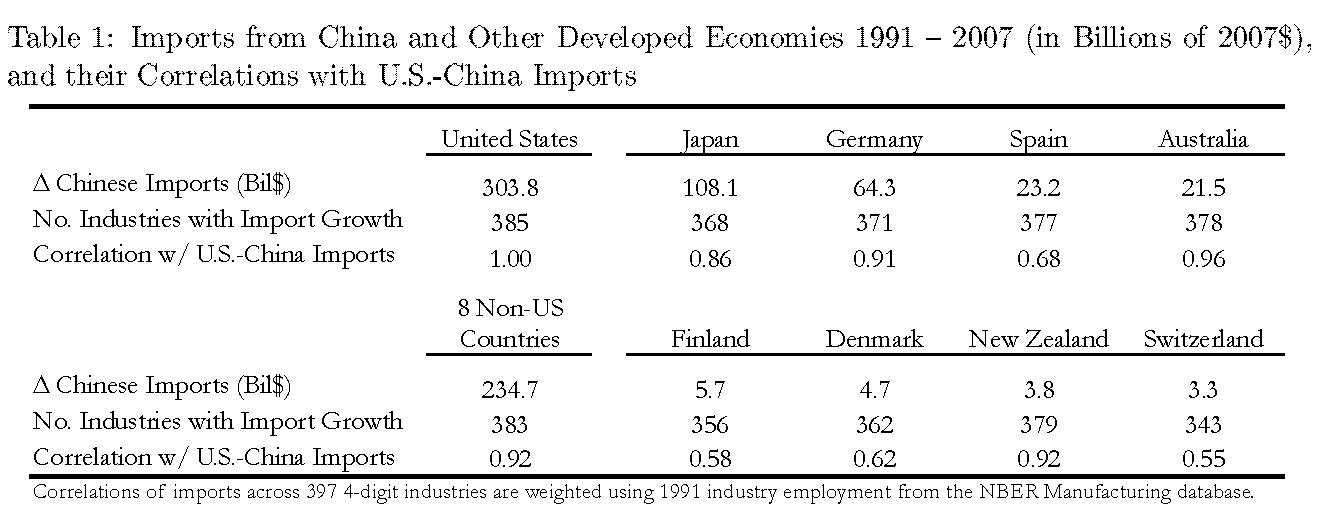
\includegraphics[scale=0.82]{AutorDornHansonTable1.jpg}
    \label{fig:Tab1}
\end{figure}
    
\end{frame}

%-------------------------------------------------------------

\begin{frame}{Instrumental Variables Strategy}

\begin{itemize}
    \item<1-> Table 1 documents the instrumental variables strategy.  Several other countries have a high correlation with the U.S. in terms of their growth in Chinese imports.
    \item<2-> There is a concern that demand changes might be correlated across high-income countries.
    \item<3-> Autor, Dorn, and Hanson (2013) also used a gravity-based strategy that used Chinese changes in revealed comparative advantage as an instrument (eliminating differences based on import demand in the purchasing country).
    \item<4-> Results did not change much, so they believe that it is not a major concern.
\end{itemize}
    
\end{frame}

%-------------------------------------------------------------

\begin{frame}{Wage Changes from Shocks}

\begin{itemize}
    \item<1-> The second term in equation (\ref{eq:xihat}) is $ \theta \hat{w}_{i} $, the endogenous change in wages in region i from trade shocks.
    \item<2-> One can estimate equation (\ref{eq:xihat}) without this term, in which case the reduced form result captures the effect on region i directly through changes in output, or indirectly through wages.
    \item<3-> Or, one can use $ \hat{w}_{i} $ as a dependent variable in a regression.
\end{itemize}
    
\end{frame}

%-------------------------------------------------------------

\begin{frame}{Change in National Industry Productivity}

\begin{itemize}
    \item<1-> The third term in equation (\ref{eq:Xi}) is $ \sum_{k} \phi_{i,k} \hat{A}_{k} $ which captures the exposure of region $ i $ to changes in national industry productivity.
    \item<2-> Autor, Dorn, and Hanson (2013, 2015) note that there is near zero correlation between technological change and exposure to trade with China across U.S. local labor markets.
    \item<3->  So there is little to no omitted variables bias from excluding this.
\end{itemize}
    
\end{frame}

%-------------------------------------------------------------

\begin{frame}{Production Capacity in Other Countries}

\begin{itemize}
    \item<1-> The fourth term in equation (\ref{eq:xihat}) is $ \sum_{k} \phi_{i,k} \sum_{i' \neq c} \rho_{i',k} \hat{A}_{i',k} $, which is the change in production capabilities in other supplying countries.
    \item<2-> If these change in response to changing supply conditions from China, excluding them from a reduced-form regression still captures the effect of changes in Chinese production capacity.
    \item<3-> The specification in (\ref{eq:xihat}) does not allow for input-output linkages.  The model will not capture the effect of a change in final goods production in the U.S. on production of intermediate inputs in the U.S..
\end{itemize}
    
\end{frame}

%-------------------------------------------------------------

\section{Labor Market Adjustment to Trade}

%-------------------------------------------------------------

\begin{frame}{Labor Market Adustment to Trade}

Effect of the China Shock is as follows:

\begin{itemize}
    \item<1-> More intense competition in product markets.
    \item<2-> Then shock is transmitted to regions that have concentrations of competing manufacturing industries.
\end{itemize}
    
\end{frame}

%-------------------------------------------------------------

\subsection{Industry Adjustment to Import Competition}

%-------------------------------------------------------------

\begin{frame}{Industry Adjustment to Import Competition}

\begin{itemize}
    \item<1-> First step is that improvements in China’s productive capacity and reductions in its trade costs will change the intensity of competition for U.S. goods, leading to a contraction in those industries subject to greater import exposure.
    \item<2-> Bernard, Jensen, and Schott (2006) find that plants facing greater increases in exposure to trade are subject to higher rates of exit.
    \item<3-> Those that survive have lowered unemployment or higher rates of changing manufacturing category.
\end{itemize}
    
\end{frame}

%-------------------------------------------------------------

\begin{frame}{Change in Labor Force}

Acemoglu, Autor, Dorn, Hanson, and Price (2016) focus on industry-level data and examine time period from 1991-2011.  They estimate the following model, similar to equation (\ref{eq:xihat}):
\begin{equation}
    \Delta L_{j,\tau} = \alpha_{\tau} + \beta_{1} \Delta IP_{j,\tau} + \gamma X_{j,0} + \varepsilon_{j,\tau}
    \label{eq:deltaL}
\end{equation}
where $ \Delta L_{j,\tau} $ is the log change in employment in industry $ j $ over time $ \tau $, $ \Delta IP_{j,\tau} $ is the log change in import penetration from China during that time, and $ X_{j,0} $ is a set of industry controls from the beginning of the period.
    
\end{frame}

%-------------------------------------------------------------

\begin{frame}{Table 2}

\begin{figure}
    \centering
    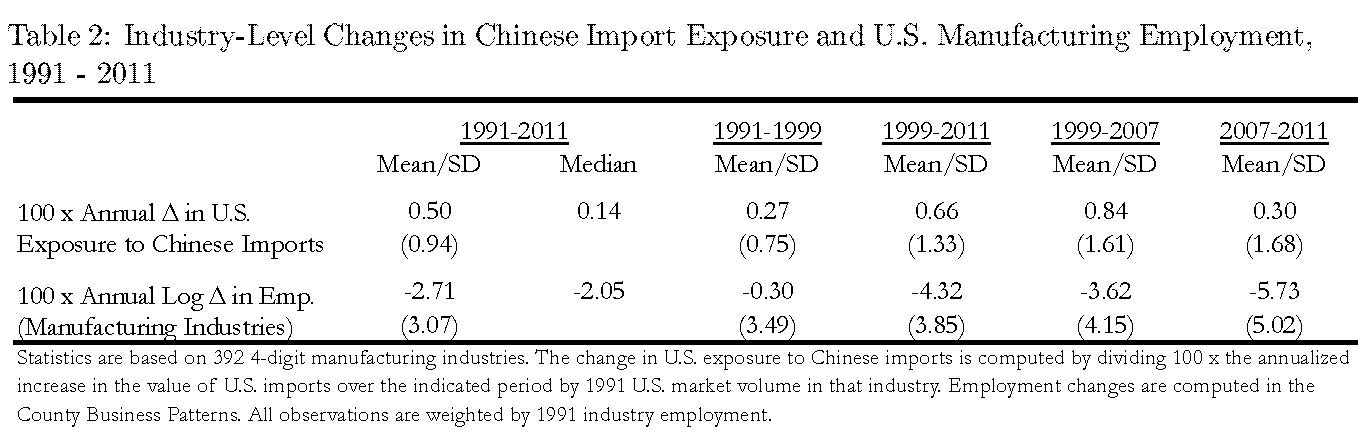
\includegraphics[scale=0.8]{AutorDornHansonTable2.jpg}
    \label{fig:Table2}
\end{figure}
    
\end{frame}

%-------------------------------------------------------------

\begin{frame}{Import Exposure and Manufacturing Unemployment}

\begin{itemize}
    \item<1-> Table 2 shows that the employment-weighted mean industry saw Chinese import penetration rise by 0.5\% a year betwen 1991-2011, which the most rapid period being between 1999-2007.
    \item<2-> The period 2007-2011 contains the global financial crisis, which saw falls in both employment and the rate of import growth.
    \item<3-> The fall in U.S. manufacturing employment also accelerated during this time.
\end{itemize}
    
\end{frame}

%-------------------------------------------------------------

\begin{frame}{Table 3}

\begin{figure}
    \centering
    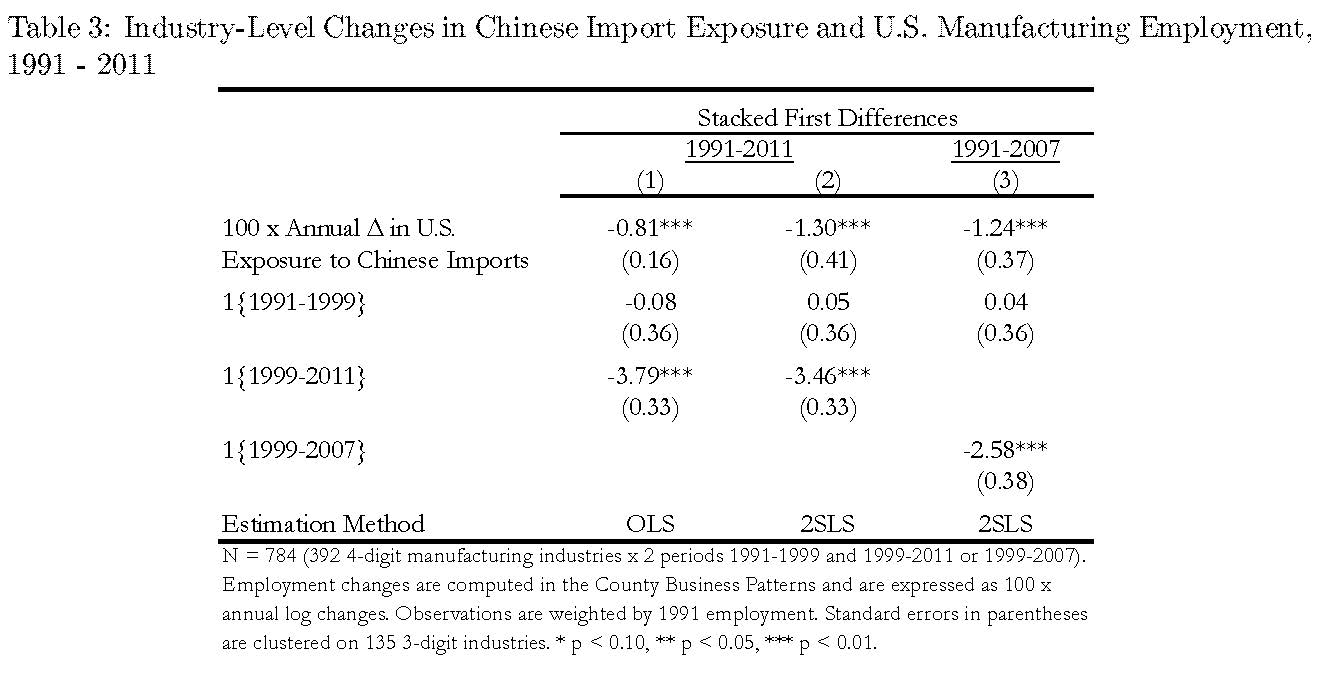
\includegraphics[scale=0.8]{AutorDornHansonTable3.jpg}
    \label{fig:Table3}
\end{figure}
    
\end{frame}

%-------------------------------------------------------------

\begin{frame}{Estimates of Equation (\ref{eq:deltaL})}

\begin{itemize}
    \item<1-> Table 3 presents estimates of equation (\ref{eq:deltaL}) in stacked first differences for 1991-1999 and 1999-2011.  The change in the import penetration ratio and the time dummies are the only regressors.
    \item<2-> Column 1 shows that the relationship between the import penetration ratio and employment is negative and highly significant over the time period.
    \item<3-> Column 2 instruments for the import penetration ratio using Chinese exports to other countries, and finds a larger effect.
    \item<3-> Column 3 restricts our attention to the period 1999-2007 using a time dummy and finds a similar effect.
\end{itemize}
    
\end{frame}

%-------------------------------------------------------------

\begin{frame}{Implications}

Clearly, exposure to Chinese imports affect industry employment, but the distributional consequences may turn on the following questions:
\begin{itemize}
    \item<1-> Do industry shocks translate into localized employment shocks?
    \item<2-> Are trade-induced employment contractions offset by employment gains elsewhere in the U.S.?
    \item<3-> Do trade adjustments occur on the employment margin, the wage margin, or both?
    \item<4-> Are the costs borne disproportionately by workers at trade-impacted firms and/or trade-impacted local labor markets, or are the costs more diffuse?
\end{itemize}
    
\end{frame}

%-------------------------------------------------------------

\subsection{Regional Employment Impacts}

%-------------------------------------------------------------

\begin{frame}{Regional Employment Impacts}

\begin{itemize}
    \item<1-> Local exposure to the China Shock varies due to the tendency of industries to cluster in a specific part of the country.  Manufacturing is disproportionately located in the Southeast and Midwest.
    \item<2-> Autor, Dorn, and Hanson (2013) divide the U.S. in commuting zones (CZs) that have the characteristics of a local labor market.
\end{itemize}
    
\end{frame}

%-------------------------------------------------------------

\begin{frame}{Figure 6a}

\begin{figure}
    \centering
    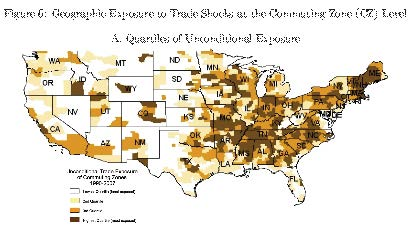
\includegraphics[scale=0.85]{AutorDornHansonFig6a.jpg}
    \label{fig:Fig6a}
\end{figure}
    
\end{frame}

%-------------------------------------------------------------

\begin{frame}{Figure 6b}

\begin{figure}
    \centering
    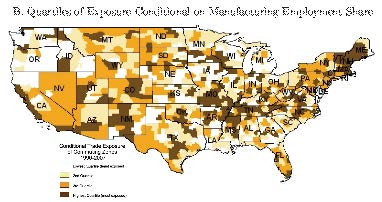
\includegraphics[scale=0.85]{AutorDornHansonFig6b.jpg}
    \label{fig:Fig6b}
\end{figure}
    
\end{frame}

%-------------------------------------------------------------

\begin{frame}{Exposure by Commuting Zone}

\begin{itemize}
    \item<1-> Panel A of Figure 6 shows the level of exposure to Chinese imports by commuting zone.
    \item<2-> Panel B shows the level of exposure conditional on manufacturing employment in the commuting zone.
    \item<3-> Mountain West seems somewhat more exposed in Panel B.
\end{itemize}
    
\end{frame}

%-------------------------------------------------------------

\begin{frame}{Table 4}

\begin{figure}
    \centering
    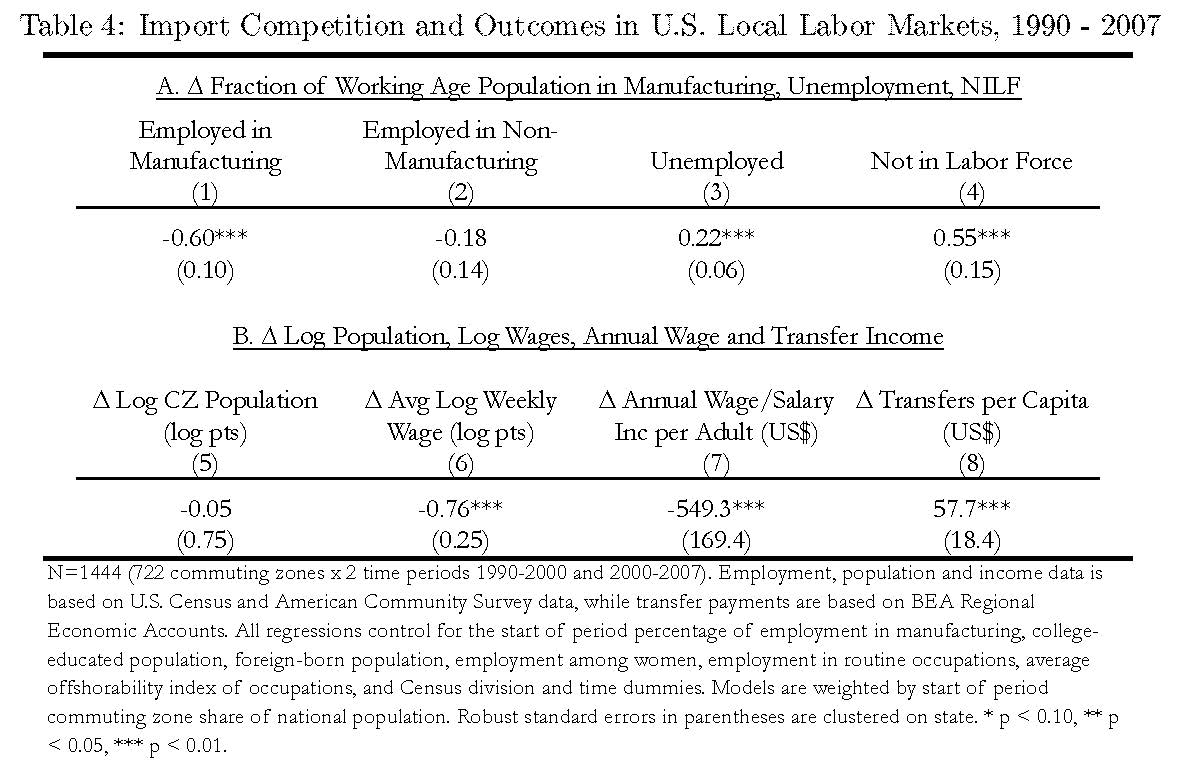
\includegraphics[scale=0.68]{AutorDornHansonTable4.jpg}
    \label{fig:Table4}
\end{figure}
    
\end{frame}

%-------------------------------------------------------------

\begin{frame}{Results by Commuting Zone}

\begin{itemize}
    \item<1-> Columns 1-4 of Table 4 shows that an increase in exposure to imports lowered manufacturing employment and raised number unemployed or not in the labor force.  A \$1000 per-worker increase in import exposure reduces the number of workers employed in manufacturing by 0.60\%.
    \item<2-> Autor, Dorn, and Hanson (2013) show that this holds for workers at all education levels.
    \item<3-> Column 5 of Table 4 shows a modest and insignificant effect of increased import exposure on working age population.
    \item<4-> Autor, Dorn, Hanson, and Song (2014) show at the individual level that there is little geographic migration in response to a trade shock.
\end{itemize}
    
\end{frame}

%-------------------------------------------------------------

\subsection{National Impacts vs. Regional Impacts}

%-------------------------------------------------------------

\begin{frame}{National Impacts vs. Regional Impacts}

\begin{itemize}
    \item<1-> These results do not make a distinction between relative losses and absolute losses.  It could be the case that a heavily affected area simply has less growth than a more sheltered area.
    \item<2-> Acemoglu, Autor, Dorn, Hanson, and Price (2016) use an expanded version of equation (\ref{eq:deltaL}) to see if adverse impacts are offset by gains elsewhere in the economy.
    \item<3-> They estimate that, had import penetration from China not grown after 1999, there would be 560,000 fewer manufacturing jobs lost (out of 5.8 million manufacturing jobs lost total).
\end{itemize}
    
\end{frame}

%-------------------------------------------------------------

\begin{frame}{Input-Output Linkages}

\begin{itemize}
    \item<1-> Previous estimates also do not take into account the upstream linkages of fall in domestic production.
    \item<2-> Acemoglu, Autor, Dorn, Hanson, and Price (2016) estimate this indirect effect using input-output matrices, come up with a job loss total of 985,000 workers in manufacturing, 2.0 million for economy as a whole.
    \item<3-> Paper notes that positive employment effects due to cheaper inputs of intermediate goods are possible in theory, but neither Pierce and Shott (2015) nor Autor, Dorn, and Hanson (2013) find an effect in this direction.
\end{itemize}
    
\end{frame}

%-------------------------------------------------------------

\subsection{Wage and Transfer Impacts}

%-------------------------------------------------------------

\begin{frame}{Wage and Transfer Impacts}

\begin{itemize}
    \item<1-> Column 6 of Table 4 showed that more trade-exposed CZs experience larger reductions in average weekly wages.
    \item<2-> Chetverikov, Larsen, and Palmer (2015) extend the analysis to a quantile regression setting and find that the wage impacts are concentrated in the bottom-four deciles.
    \item<3-> An increase of \$1000 in exposure to Chinese imports reduces the earnings of the average still-employed worker (earning \$40,000 a year) by about 0.76 log-points of wage, or around \$213 a year.
    \item<4-> A reduction in employment and wages in a CZ also results in an increase in transfer benefits (specifically, unemployment insurance and Trade Adjustment Assistance).  Also, a prolonged downturn increases the number of people who qualify for means-tested benefits (TANF, food stamps, etc.).
\end{itemize}
    
\end{frame}

%-------------------------------------------------------------

\begin{frame}{Figure 7}

\begin{figure}
    \centering
    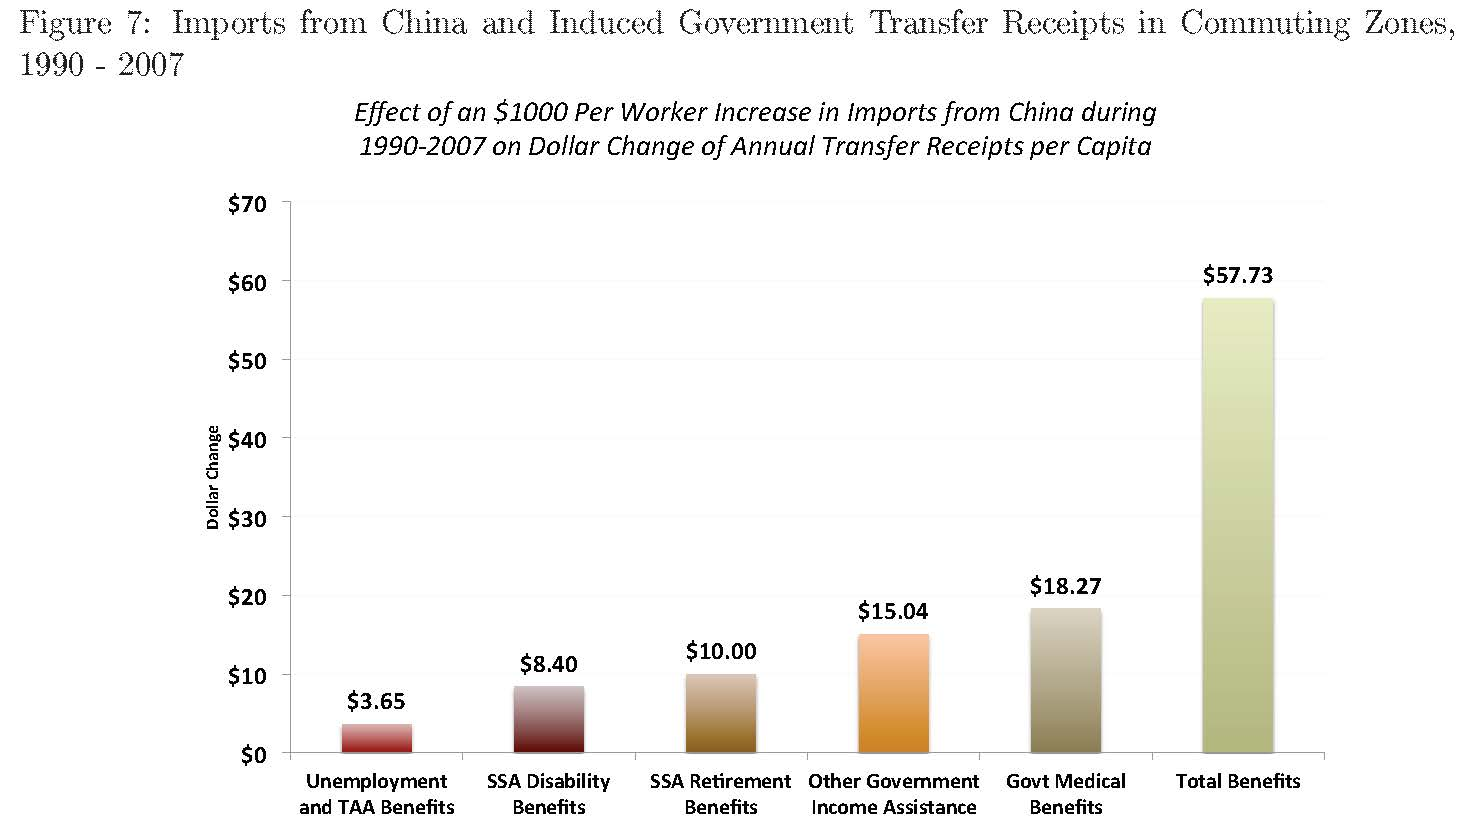
\includegraphics[scale=0.7]{AutorDornHansonFig7.jpg}
    \label{fig:Fig7}
\end{figure}
    
\end{frame}

%-------------------------------------------------------------

\begin{frame}{Impacts on Transfer Programs}

\begin{itemize}
    \item<1-> Figure 7 shows the impact of an increase of \$1000 in Chinese import exposure on increases in government transfer programs.
    \item<2-> TAA and unemployment are actually the smallest category in this figure.  Disability, retirement, and health care benefits, which are designed to be more permanent, are actually the largest categories.
\end{itemize}
    
\end{frame}

%-------------------------------------------------------------

\subsection{Worker Level Impacts}

%-------------------------------------------------------------

\begin{frame}{Worker Level Impacts}

\begin{itemize}
    \item<1-> Preceding analysis does not make a distinction between workers in a locality that is exposed to trade and workers at a particular firm that is exposed to trade.
    \item<2-> In a Heckscher-Ohlin world, all workers of a particular skill level or type should be equally affect.  With imperfect labor mobility, trade shocks could have heterogeneous impacts within groups.
    \item<3-> Autor, Dorn, Hanson, and Song (2014) use longitudinal data from the U.S. S.S.A.  Workers whose 1991 industry of employment became more highly exposed to imports experience lower earnings and higher job churn than workers with similar characteristics.
    \item<4-> Non-trade labor literature on job loss suggests that displacement destroys industry-specific human capital.  Relatedly, when workers lose jobs, other firms in related industries may be facing the same challenges and not hiring.
\end{itemize}
    
\end{frame}

%-------------------------------------------------------------

\begin{frame}{Figure 8}

\begin{figure}
    \centering
    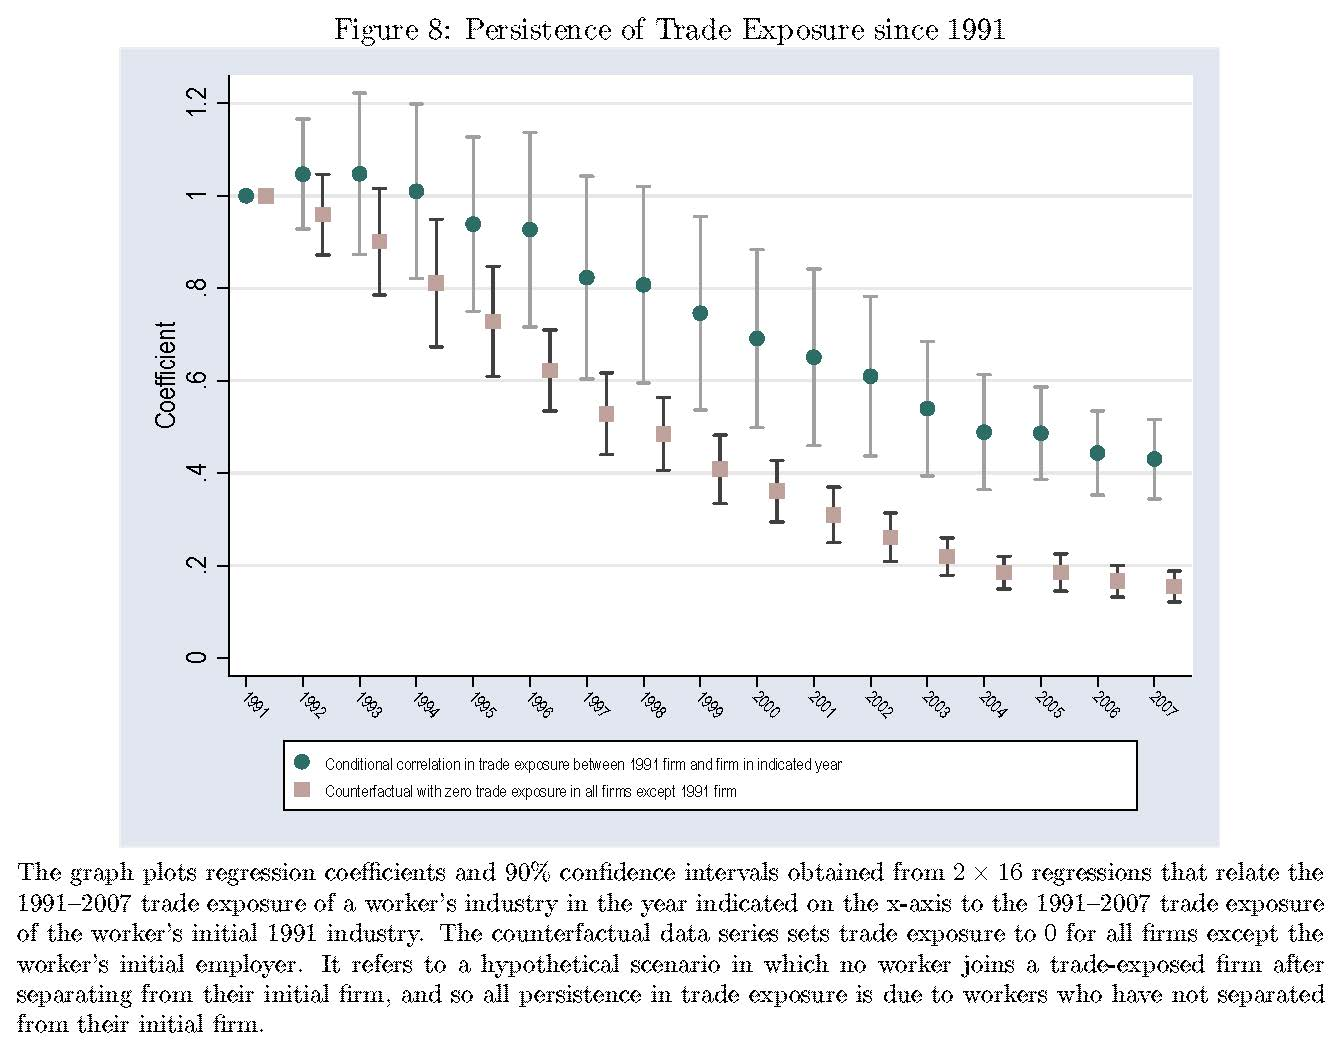
\includegraphics[scale=0.53]{AutorDornHansonFig8.jpg}
    \label{fig:Fig8}
\end{figure}
    
\end{frame}

%-------------------------------------------------------------

\begin{frame}{Persistence of Trade Exposure}

\begin{itemize}
    \item<1-> Figure 8 shows the correlation between a worker’s trade exposure at the 1991 job vs. trade exposure at jobs in subsequent years.
    \item<2-> Stays high at first (relatively few workers having left initial job) and gradually falls to 0.43 (still significant) in 2007.
    \item<3-> Counter factual analysis shows what would happen if worker left trade-exposed field after first job separation.  Falls more rapidly and ends at 0.17 in 2007.
    \item<4-> Implication is that, if workers left manufacturing immediately upon losing job, they would have about 60\% less exposure to trade shocks.  But they tend to persist in trade exposed fields.  
\end{itemize}
    
\end{frame}

%-------------------------------------------------------------

\begin{frame}{Variation by Income Level}

\begin{itemize}
    \item<1-> Substantial heterogeneity exists at the income level.
    \item<2-> Workers in the top earning tercile are more likely to relocate out of manufacturing after a trade shock than those in the bottom tercile.
    \item<3-> Their earnings loss is not significantly different from workers in less trade-exposed industries.
\end{itemize}
    
\end{frame}

%-------------------------------------------------------------

\section{(Re)Assessing the Gains from Trade}

%-------------------------------------------------------------

\begin{frame}{(Re)Assessing the Gains from Trade}

\begin{itemize}
    \item<1-> China experienced one of the most substantial and rapid accumulations of wealth in human history, which resulted in a huge surge in exports to the U.S. (and other countries).
    \item<2-> Standard trade model predicts that jobs in the U.S. should reallocate between tradeable sectors of the economy (with some limited movement to the non-tradeable sectors).  Limited impact on aggregate employment.
    \item<3-> This has not happened in the U.S. – workers in import-competing sectors have largely moved either to non-tradeable sectors or out of the labor force.  Big negative consequences for highly exposed labor markets.
\end{itemize}
    
\end{frame}

%-------------------------------------------------------------

\begin{frame}{Concentrated Effects}

\begin{itemize}
    \item<1-> Effect seems to be heterogeneous by wage.  In response to a trade shock, a low wage worker will experience a proportionately larger decrease in annual and lifetime earnings, a diminished ability to exit the job before the shock hits, and a greater likelihood of exiting the labor market entirely than a high wage worker.
    \item<2-> Concentration of trade exposed industries in certain local labor markets hinders movement of workers.  Hence, a trade shock may impose larger adjustment costs than is typically assumed by the literature.
    \item<3-> China Shock seemed to diminish by the time it was recognized.  Wages are rising in China, exports are increasingly moving from cheap manufactures to areas where it has a technological prowess.  Trade war and COVID-19 also bringing this era to an end.
\end{itemize}
    
\end{frame}

%-------------------------------------------------------------

\section{Autor, Dorn, and Hanson Oeuvre}

%-------------------------------------------------------------

\begin{frame}{Autor, Dorn, and Hanson Oeuvre}

This paper is a sort of compendium of a series of papers that Autor, Dorn, Hanson, and various co-authors have written on this topic.
\begin{itemize}
    \item<1-> Original paper:  David, H., David Dorn, and Gordon H. Hanson. ``The geography of trade and technology shocks in the United States." \emph{American Economic Review} 103, no. 3 (2013): 220-25.
    \item<2-> Worker level effects:  Autor, David H., David Dorn, Gordon H. Hanson, and Jae Song. ``Trade adjustment: Worker-level evidence." \emph{The Quarterly Journal of Economics} 129, no. 4 (2014): 1799-1860.
    \item<3-> Trade and technology:  Autor, David H., David Dorn, and Gordon H. Hanson. ``Untangling trade and technology: Evidence from local labour markets." \emph{The Economic Journal} 125, no. 584 (2015): 621-646.  
\end{itemize}
    
\end{frame}

%-------------------------------------------------------------

\begin{frame}{Autor, Dorn, and Hanson Oeuvre}

\begin{itemize}
    \item<1-> Political Effects: Dorn, David, Gordon Hanson, and Kaveh Majlesi. ``Importing political polarization? The electoral consequences of rising trade exposure." \emph{American Economic Review} 110, no. 10 (2020): 3139-83.
    \item<2-> National employment rate:  Acemoglu, Daron, David Autor, David Dorn, Gordon H. Hanson, and Brendan Price. ``Import competition and the great US employment sag of the 2000s." \emph{Journal of Labor Economics} 34, no. S1 (2016): S141-S198.
    \item<3-> Marriage markets: Dorn, David, and Gordon Hanson. ``When work disappears: Manufacturing decline and the falling marriage market value of young men." \emph{American Economic Review: Insights} 1, no. 2 (2019): 161-78.  
\end{itemize}
    
\end{frame}

%-------------------------------------------------------------

\end{document}